% start preamble -------------------------------------------------------------
\documentclass{article}
\usepackage{amsmath, amsthm, amssymb, amsfonts}
\usepackage{thmtools}
\usepackage{graphicx}
\usepackage{setspace}
\usepackage{geometry}
\usepackage{float}
\usepackage{hyperref}
\usepackage[utf8]{inputenc}
\usepackage[english]{babel}
\usepackage{framed}
\usepackage[dvipsnames]{xcolor}
\usepackage{tcolorbox}
\usepackage{ dsfont }
\usepackage[math]{cellspace}
\usepackage{tikz}
\usetikzlibrary{arrows, automata, positioning}
\usepackage{ multicol }

\setlength\cellspacetoplimit{3pt}
\setlength\cellspacebottomlimit{3pt}
\colorlet{LightGray}{White!90!Periwinkle}
\colorlet{LightOrange}{Orange!15}
\colorlet{LightGreen}{Green!15}

\graphicspath{ {./pictures/} }

\newcommand{\HRule}[1]{\rule{\linewidth}{#1}}

% end preamble -------------------------------------------------------------------

% set node types for tikz
\tikzset{
  treenode/.style = {align=center, inner sep=0pt, text centered,
    font=\sffamily},
  ch/.style = {treenode, circle, black, draw=black, 
    text width=1.5em, very thick}
}
\begin{document}

% ------------------------------------------------------------------------------
% Cover Page and ToC
% ------------------------------------------------------------------------------

\title{ \normalsize \textsc{}
		\\ [2.0cm]
		\HRule{1.5pt} \\
		\LARGE \textbf{\uppercase{ AuD Übungsblatt Nr. 9 }
        \HRule{2.0pt} \\ [0.6cm] \LARGE{ Hannes Albert } \vspace*{10\baselineskip}}
		}
\date{Juni 2023}
\author{\textbf{} \\
		Gruppe: 36 \\
		Tutor: Julian Eulenburg }

\maketitle
\newpage
\section*{H1}
\noindent a) 
\begin{multicols}{3}
\ $\overset{insert(T, 4)}{\rightarrow}$

\begin{tikzpicture}[baseline, ->,>=stealth',level/.style={sibling distance = 5cm/#1,
  level distance = 1.5cm}] 
\node [ch] {4}
; 
\end{tikzpicture}
\ $\overset{insert(T, 6)}{\rightarrow}$
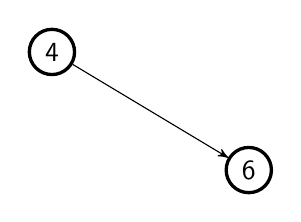
\begin{tikzpicture}[baseline, ->,>=stealth',level/.style={sibling distance = 5cm/#1,
  level distance = 1.5cm}] 
\node [ch] {4}
child [missing]
child{ node [ch] {6}}
; 
\end{tikzpicture}
\ $\overset{zig(T, 6)}{\rightarrow}$
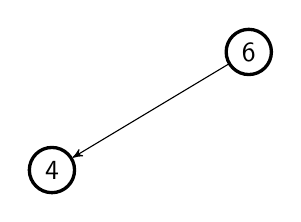
\begin{tikzpicture}[baseline, ->,>=stealth',level/.style={sibling distance = 5cm/#1,
  level distance = 1.5cm}] 
\node [ch] {6}
child{ node [ch] {4}}
child [missing]
; 
\end{tikzpicture}
\end{multicols}

\bigskip
\begin{multicols}{2}
$\overset{insert(T, 8)}{\rightarrow}$
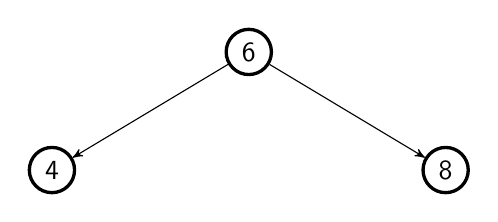
\begin{tikzpicture}[baseline, ->,>=stealth',level/.style={sibling distance = 5cm/#1,
  level distance = 1.5cm}] 
\node [ch] {6}
child{ node [ch] {4}}
child { node [ch] {8}}
; 
\end{tikzpicture}
\ $\overset{zig(T, 8)}{\rightarrow}$
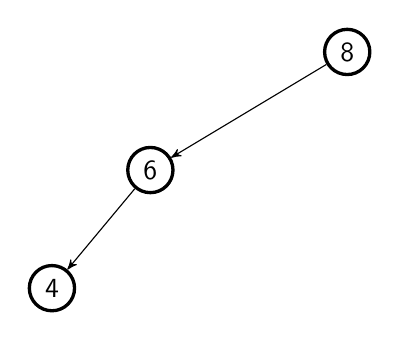
\begin{tikzpicture}[baseline, ->,>=stealth',level/.style={sibling distance = 5cm/#1,
  level distance = 1.5cm}] 
\node [ch] {8}
child{ node [ch] {6}
    child { node [ch] {4}}
    child [missing]
    }
child [missing]
;
\end{tikzpicture}
\end{multicols}

\bigskip
\begin{multicols}{2}
\ $\overset{insert(T, 1)}{\rightarrow}$
\begin{tikzpicture}[baseline, ->,>=stealth',level/.style={sibling distance = 5cm/#1,
level distance = 1.5cm}] 
\node [ch] {8}
child{ node [ch] {6}
child{ node [ch] {4} 
            child{ node [ch] {1}
         }
            child [missing]
        }
        child [missing] }
child [missing]
;
\end{tikzpicture}
\ $\overset{zigZig(T, 1)}{\rightarrow}$
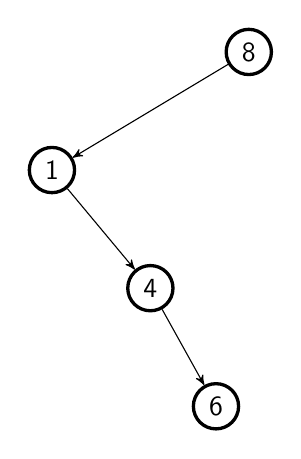
\begin{tikzpicture}[baseline, ->,>=stealth',level/.style={sibling distance = 5cm/#1,
level distance = 1.5cm}] 
\node [ch] {8}
child{ node [ch] {1}
child [missing]
child{ node [ch] {4}
            child [missing]
            child{ node [ch] {6}}
    }}
child [missing]
;
\end{tikzpicture}
\end{multicols}

\bigskip
$\overset{zig(T, 1)}{\rightarrow}$
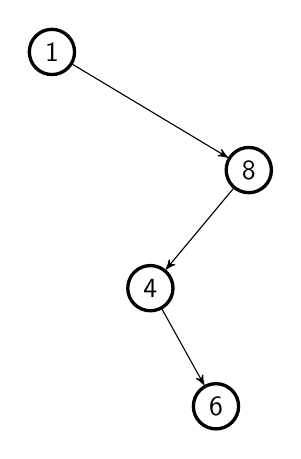
\begin{tikzpicture}[baseline, ->,>=stealth',level/.style={sibling distance = 5cm/#1,
level distance = 1.5cm}] 
\node [ch] {1}
child [missing]
child{ node [ch] {8}
child{ node [ch] {4}
            child [missing]
            child{ node [ch] {6}}
    }
child [missing]
}
;
\end{tikzpicture}
$\overset{insert(T, 5)}{\rightarrow}$
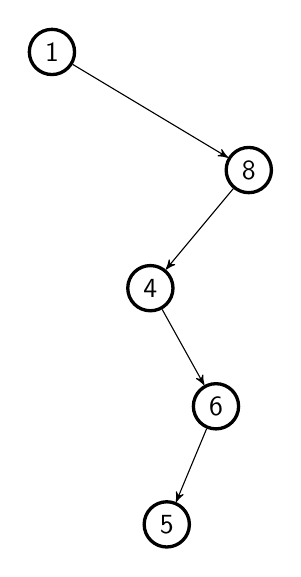
\begin{tikzpicture}[baseline, ->,>=stealth',level/.style={sibling distance = 5cm/#1,
level distance = 1.5cm}] 
\node [ch] {1}
child [missing]
child{ node [ch] {8}
child{ node [ch] {4}
            child [missing]
            child{ node [ch] {6}
                child { node [ch] {5}}
                child [missing]
            }
    }
child [missing]
}
;
\end{tikzpicture}

\bigskip
$\overset{zigZag(T, 5)}{\rightarrow}$
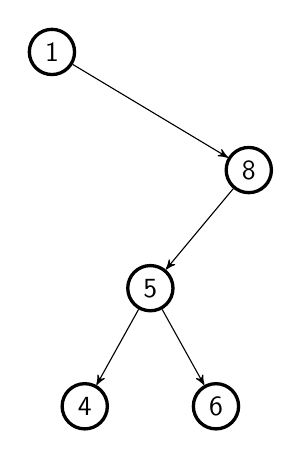
\begin{tikzpicture}[baseline, ->,>=stealth',level/.style={sibling distance = 5cm/#1,
level distance = 1.5cm}] 
\node [ch] {1}
child [missing]
child{ node [ch] {8}
child{ node [ch] {5}
            child{ node [ch] {4}}
            child{ node [ch] {6}}
    }
child [missing]
}
;
\end{tikzpicture}
\bigskip
$\overset{zigZag(T, 5)}{\rightarrow}$
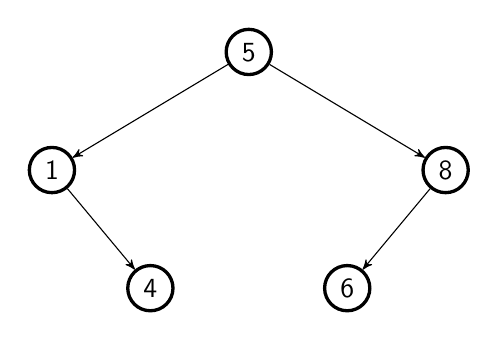
\begin{tikzpicture}[baseline, ->,>=stealth',level/.style={sibling distance = 5cm/#1,
level distance = 1.5cm}] 
\node [ch] {5}
child{ node [ch] {1}
    child [missing]
    child{ node [ch] {4}}}
child{ node [ch] {8}
    child{ node [ch] {6}}
    child [missing]}
;
\end{tikzpicture}

\bigskip
$\overset{insert(T, 7)}{\rightarrow}$
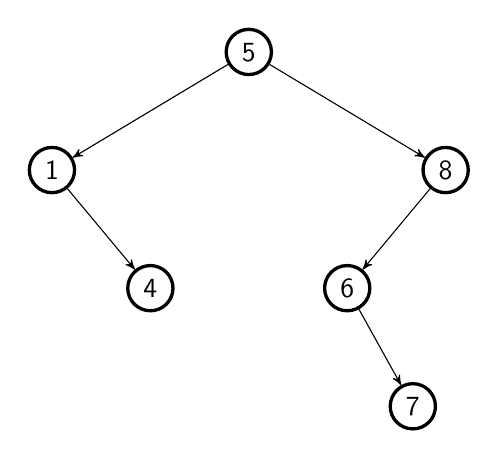
\begin{tikzpicture}[baseline, ->,>=stealth',level/.style={sibling distance = 5cm/#1,
level distance = 1.5cm}] 
\node [ch] {5}
child{ node [ch] {1}
    child [missing]
    child{ node [ch] {4}}}
child{ node [ch] {8}
    child{ node [ch] {6}
        child [missing]
        child{node [ch] {7}}
    }
    child [missing]}
;
\end{tikzpicture}

\bigskip
$\overset{zigZag(T, 7)}{\rightarrow}$
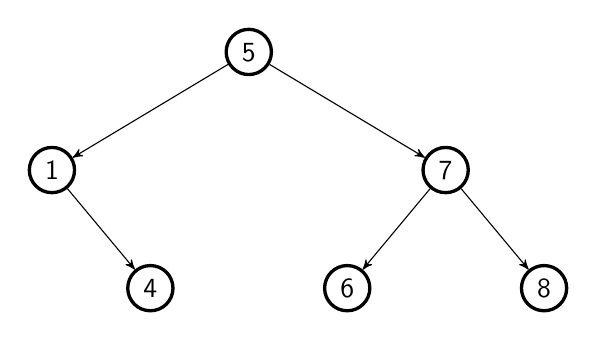
\begin{tikzpicture}[baseline, ->,>=stealth',level/.style={sibling distance = 5cm/#1,
level distance = 1.5cm}] 
\node [ch] {5}
child{ node [ch] {1}
    child [missing]
    child{ node [ch] {4}}}
child{ node [ch] {7}
    child{ node [ch] {6}}
    child{node [ch] {8}}}
;
\end{tikzpicture}
\bigskip
$\overset{zig(T, 7)}{\rightarrow}$
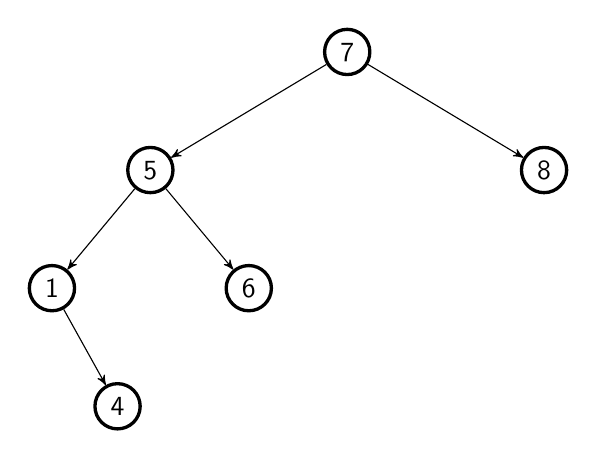
\begin{tikzpicture}[baseline, ->,>=stealth',level/.style={sibling distance = 5cm/#1,
level distance = 1.5cm}] 
\node [ch] {7}
child{ node [ch] {5}
    child{ node [ch] {1}
        child [missing]
        child{ node [ch] {4}}
    }
    child{ node [ch] {6}}}
child{ node [ch] {8}}
;
\end{tikzpicture}
\bigskip
$\overset{insert(T, 9)}{\rightarrow}$
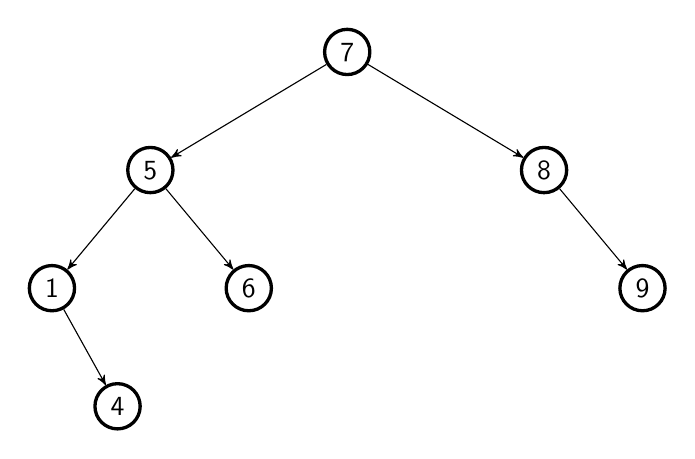
\begin{tikzpicture}[baseline, ->,>=stealth',level/.style={sibling distance = 5cm/#1,
level distance = 1.5cm}] 
\node [ch] {7}
child{ node [ch] {5}
    child{ node [ch] {1}
        child [missing]
        child{ node [ch] {4}}
    }
    child{ node [ch] {6}}}
child{ node [ch] {8}
    child [missing]
    child{ node [ch] {9}}
}
;
\end{tikzpicture}
\bigskip
$\overset{zigZig(T, 9)}{\rightarrow}$
\begin{tikzpicture}[baseline, ->,>=stealth',level/.style={sibling distance = 5cm/#1,
level distance = 1.5cm}] 
\node [ch] {9}
child{ node [ch] {8}
    child{ node [ch] {7}
        child{ node [ch] {5}
            child{node [ch] {1}
            child [missing]
            child{ node [ch] {4}}}
            child {node [ch] {6}}}
        child [missing]}    
    child [missing]}
child [missing]
;
\end{tikzpicture}
\bigskip
$\overset{insert(T, 12)}{\rightarrow}$
\begin{tikzpicture}[baseline, ->,>=stealth',level/.style={sibling distance = 5cm/#1,
level distance = 1.5cm}] 
\node [ch] {9}
child{ node [ch] {8}
    child{ node [ch] {7}
        child{ node [ch] {5}
            child{node [ch] {1}
            child [missing]
            child{ node [ch] {4}}}
            child {node [ch] {6}}}
        child [missing]}    
    child [missing]}
child{ node [ch] {12}}
;
\end{tikzpicture}
\bigskip
$\overset{zig(T, 12)}{\rightarrow}$
\begin{tikzpicture}[baseline, ->,>=stealth',level/.style={sibling distance = 5cm/#1,
level distance = 1.5cm}] 
\node [ch] {12}
child{ node [ch] {9}
    child{ node [ch] {8}
        child{ node [ch] {7}
            child{node [ch] {5}
                child{ node [ch] {1}
                child [missing]
            child{ node [ch] {4}}}
            child{ node [ch] {6}}}
        child [missing]}
        child [missing]}    
    child [missing]}
    child [missing]
;
\end{tikzpicture}

\noindent b) \\ 
Search(T, 5): \\ 
$\overset{zigZig(T, 5)}{\rightarrow}$
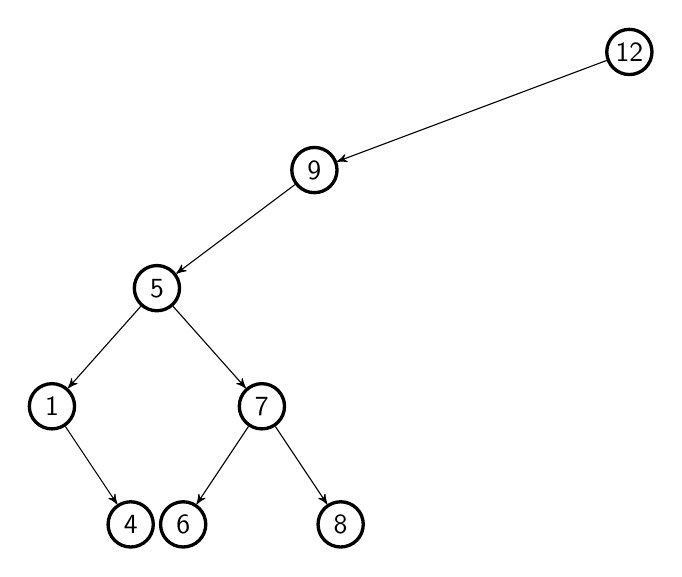
\begin{tikzpicture}[baseline, ->,>=stealth',level/.style={sibling distance = 8cm/#1,
level distance = 1.5cm}] 
\node [ch] {12}
child{ node [ch] {9}
    child{ node [ch] {5}
        child{ node [ch] {1}
        child [missing]
        child{ node [ch] {4}}}
        child{ node [ch] {7}
            child{ node [ch] {6}}
        child{ node [ch] {8}}}
    }
    child [missing]
}    
child [missing]
;
\end{tikzpicture}
\newpage
$\overset{zigZig(T, 5)}{\rightarrow}$
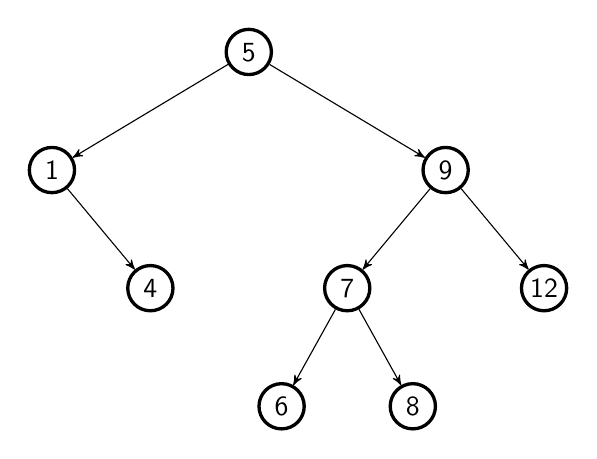
\begin{tikzpicture}[baseline, ->,>=stealth',level/.style={sibling distance = 5cm/#1,
level distance = 1.5cm}] 
\node [ch] {5}
child{ node [ch] {1}
    child [missing]
    child{node [ch] {4}}}
child{ node [ch] {9}
    child{node [ch] {7}
        child{node [ch] {6}}
        child{node [ch] {8}}}
    child{node [ch] {12}}}
;
\end{tikzpicture}

\bigskip
Delete(T, 9):

$\overset{zig(T, 9)}{\rightarrow}$
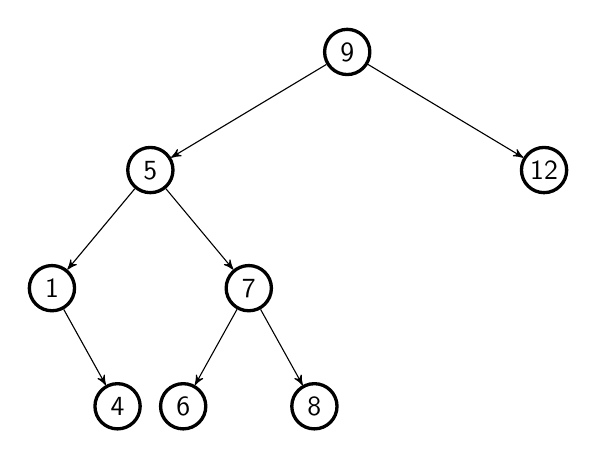
\begin{tikzpicture}[baseline, ->,>=stealth',level/.style={sibling distance = 5cm/#1,
level distance = 1.5cm}] 
\node [ch] {9}
child{ node [ch] {5}
    child{node [ch] {1}
        child [missing]
        child{node [ch] {4}}}
    child{node [ch] {7}
        child{ node [ch] {6}}
    child{ node [ch] {8}}}}
child{ node [ch] {12}}
;
\end{tikzpicture}


\bigskip
L = 
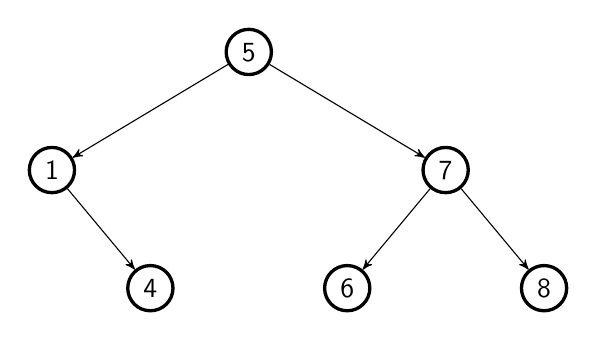
\begin{tikzpicture}[baseline, ->,>=stealth',level/.style={sibling distance = 5cm/#1,
level distance = 1.5cm}] 
\node [ch] {5}
child{ node [ch] {1}
    child [missing]
    child{ node [ch] {4}}}
child{ node [ch] {7}
    child{ node [ch] {6}}
    child{ node [ch] {8}}}
;
\end{tikzpicture}
R = 

\begin{tikzpicture}[baseline, ->,>=stealth',level/.style={sibling distance = 5cm/#1,
level distance = 1.5cm}] 
\node [ch] {12}
;
\end{tikzpicture}


\bigskip
$\overset{zigZig(L, 8)}{\rightarrow}$
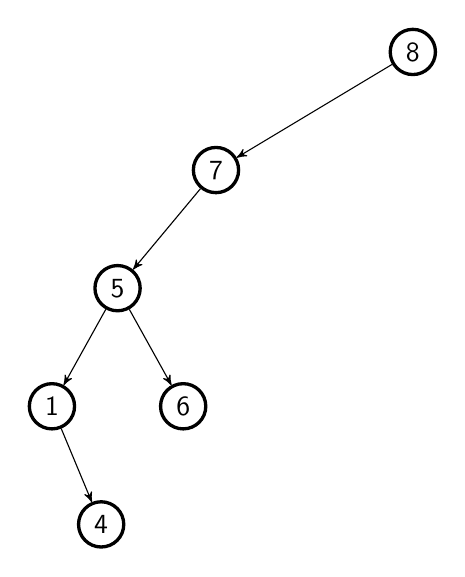
\begin{tikzpicture}[baseline, ->,>=stealth',level/.style={sibling distance = 5cm/#1,
level distance = 1.5cm}] 
\node [ch] {8}
child{ node [ch] {7}
    child{ node [ch] {5}
        child{ node [ch] {1}
        child [missing]
        child{node [ch] {4}}}
        child{ node [ch] {6}}}
    child [missing]}
child [missing]
;
\end{tikzpicture}


\bigskip
R an L anhängen:
\begin{tikzpicture}[baseline, ->,>=stealth',level/.style={sibling distance = 5cm/#1,
level distance = 1.5cm}] 
\node [ch] {8}
child{ node [ch] {7}
    child{ node [ch] {5}
        child{ node [ch] {1}
        child [missing]
        child{node [ch] {4}}}
        child{ node [ch] {6}}}
    child [missing]}
    child{ node [ch] {12}} 
;
\end{tikzpicture}

\newpage
\section*{H2}
\noindent a) \\
4 ist unser akzeptierender Zustand: 

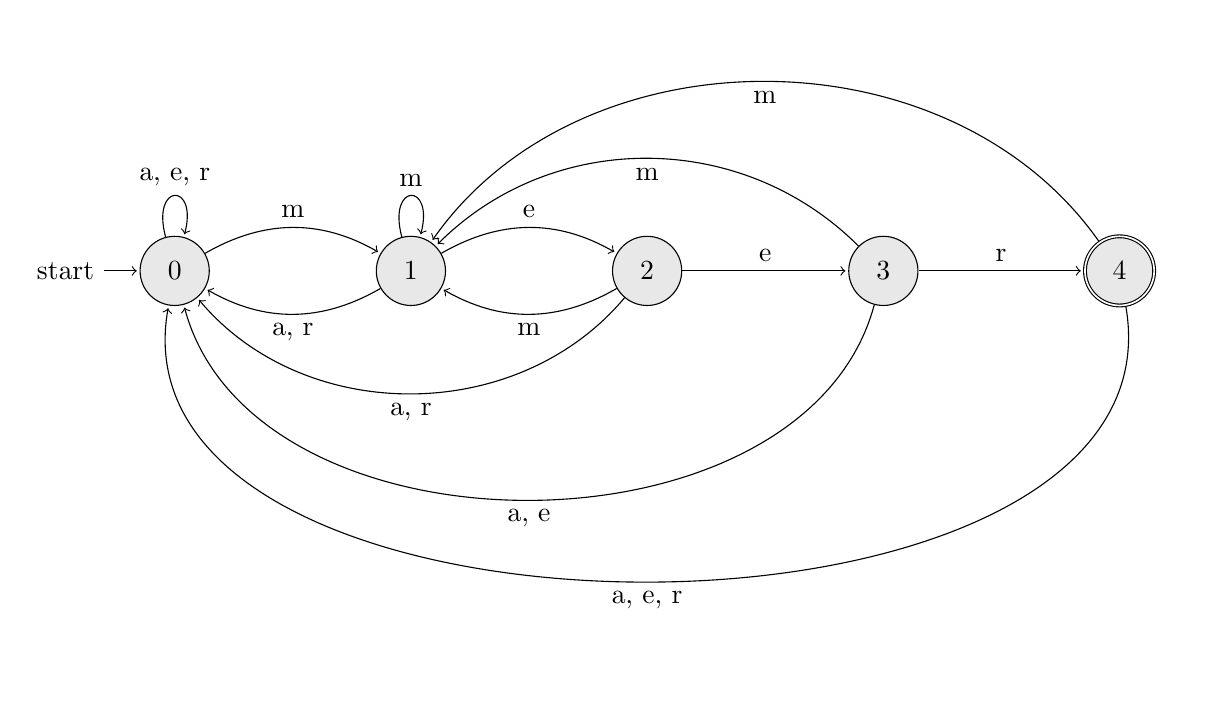
\begin{tikzpicture}[shorten >=1pt,node distance=3cm,on grid,auto]
  \tikzstyle{every state}=[fill={rgb:black,1;white,10}]

  \node[state,initial]            (0)               {$0$};
  \node[state]                    (1) [right of=0]  {$1$};
  \node[state]                    (2) [right of=1]  {$2$};
  \node[state]                    (3) [right of=2]  {$3$};
  \node[state, accepting]         (4) [right of=3]  {$4$};

  \path[->]
  (0) edge  [loop above]  node {a, e, r} ()
  (0) edge  [bend left]   node {m}  (1)
  (1) edge  [loop above]  node {m}  ()
  (1) edge  [bend left]  node {a, r} (0)
  (1) edge  [bend left]              node {e} (2)
  (2) edge  [bend left]              node {m} (1)
  (2) edge                node {e} (3)
  (2) edge  [bend left=50]              node {a, r} (0)
  (3) edge  [bend left=75]              node {a, e} (0)
  (3) edge  [bend right=45]              node {m} (1)
  (3) edge               node {r} (4)
  (4) edge [bend left=100]    node {a, e, r} (0)
  (4) edge [bend right=55]               node {m} (1);
\end{tikzpicture}

\noindent b) \\ 
\begin{table}[h!]  
\begin{center}  
\begin{tabular}{|l|c|c|r|}  
    \textbf{sft} & \textbf{T[sft]} & \textbf{st} & L\\  
\hline  
    0 & a & 0 & []\\  
    1 & m & 1 & []\\  
    2 & e & 2 & []\\  
    3 & r & 0 & []\\  
    4 & m & 1 & []\\  
    5 & e & 2 & []\\  
    6 & m & 1 & []\\  
    7 & e & 2 & []\\  
    8 & e & 3 & []\\  
    9 & r & 4 & [6]\\  
    10 & m & 1 & [6]\\  
    11 & a & 0 & [6]\\  
    12 & m & 1 & [6]\\  
    13 & e & 2 & [6]\\  
    14 & e & 3 & [6]\\  
    15 & r & 4 & [6, 12]\\  
    16 & a & 0 & [6, 12]\\  
\end{tabular}  
\end{center}  
\end{table}

\newpage
\section*{H3}
\noindent i) 
\begin{table}[h!]  
\begin{center}  
\begin{tabular}{|l|c|c|r|}  
    \textbf{Iteration} & \textbf{u} & \textbf{v} & Q\\  
\hline  
    0 & - & $\square$ & [14]\\  
    1 & 14 & 11, 13, 15, 20 & [11, 13, 15, 20]\\  
    2 & 11 & 4 & [13, 15, 20, 4]\\  
    3 & 13 & 7, 18 & [15, 20, 4, 7, 18]\\  
    4 & 15 & $\square$ & [20, 4, 7, 18]\\  
    5 & 20 & 17, 19 & [4, 7, 18, 17, 19]\\ 
    6 & 4 & $\square$ & [7, 18, 17, 19]\\  
    7 & 7 & $\square$ & [18, 17, 19]\\  
    8 & 18 & $\square$ & [17, 19]\\  
    9 & 17 & $\square$ & [19]\\  
    10 & 19 & 9 & [9]\\  
    11 & 9 & 8 & [8]\\  
    12 & 8 & $\square$ & []\\  
\end{tabular}  
\end{center}  
\end{table}

\noindent ii)

\bigskip
$G^{14}_{Pred}$ = \\  
\smallskip
\begin{tikzpicture}[baseline, ->,>=stealth',level/.style={sibling distance = 5cm/#1,
level distance = 1.5cm}] 
\node [ch] {14}
child{ node [ch] {11}
child{ node [ch] {4}}}
child{ node [ch] {13}
    child{ node [ch] {7}}
    child{ node [ch] {18}}}
child{ node [ch] {15}}
child{ node [ch] {20}
    child{node [ch] {17}}
    child{node [ch] {19}
        child{node [ch] {9}
child{node [ch] {8}}}}}
;
\end{tikzpicture}

\newpage
\noindent c) \\ 
Folgende vier Kanten erfüllen die gewünschten Eigenschaften: \\ 
\begin{itemize}
    \item \{10, 16\}
    \item \{16, 18\}
    \item \{12, 17\} 
    \item \{1, 4\}
\end{itemize}

\bigskip
Hier nochmal die Kanten in Blau eingefügt:

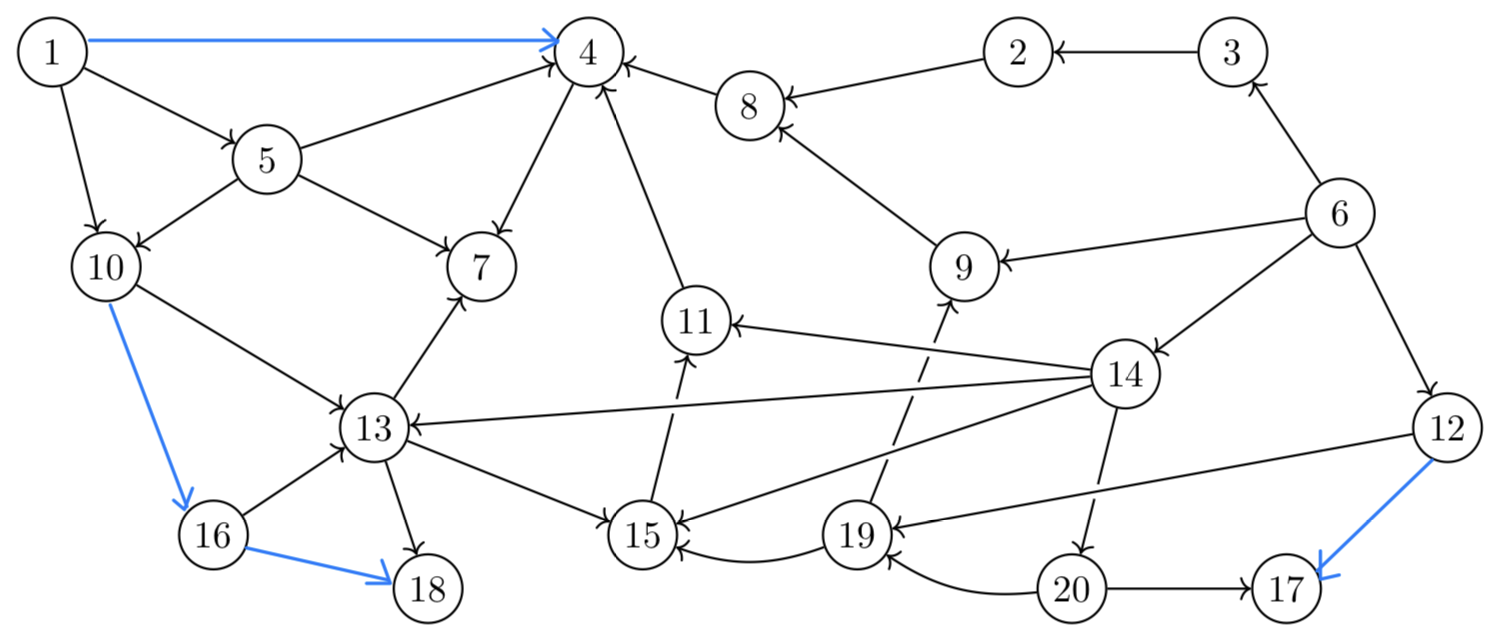
\includegraphics[scale=0.5]{graph}
\end{document}
